% -*- latex -*-
%%%%%%%%%%%%%%%%%%%%%%%%%%%%%%%%%%%%%%%%%%%%%%%%%%%%%%%%%%%%%%%%
%%%%%%%%%%%%%%%%%%%%%%%%%%%%%%%%%%%%%%%%%%%%%%%%%%%%%%%%%%%%%%%%
%%%%
%%%% This text file is part of the source of 
%%%% `Parallel Programming in MPI and OpenMP'
%%%% by Victor Eijkhout, copyright 2012-7
%%%%
%%%% mpi-ptp.tex : about point-to-point communication
%%%%
%%%%%%%%%%%%%%%%%%%%%%%%%%%%%%%%%%%%%%%%%%%%%%%%%%%%%%%%%%%%%%%%
%%%%%%%%%%%%%%%%%%%%%%%%%%%%%%%%%%%%%%%%%%%%%%%%%%%%%%%%%%%%%%%%

\Level 0 {Distributed computing and distributed data}

One reason for using MPI is that sometimes you need to work on
more data than can fit in the memory of a single processor.
With distributed memory, each processor then gets a part
of the whole data structure and only works on that.

So let's say we have a large array, and we want to
distribute the data over the processors.
That means that, with \n{p} processes and \n{n}~elements
per processor, we have a total of $\n{n}\cdot\n{p}$ elements.

\begin{figure}[ht]
  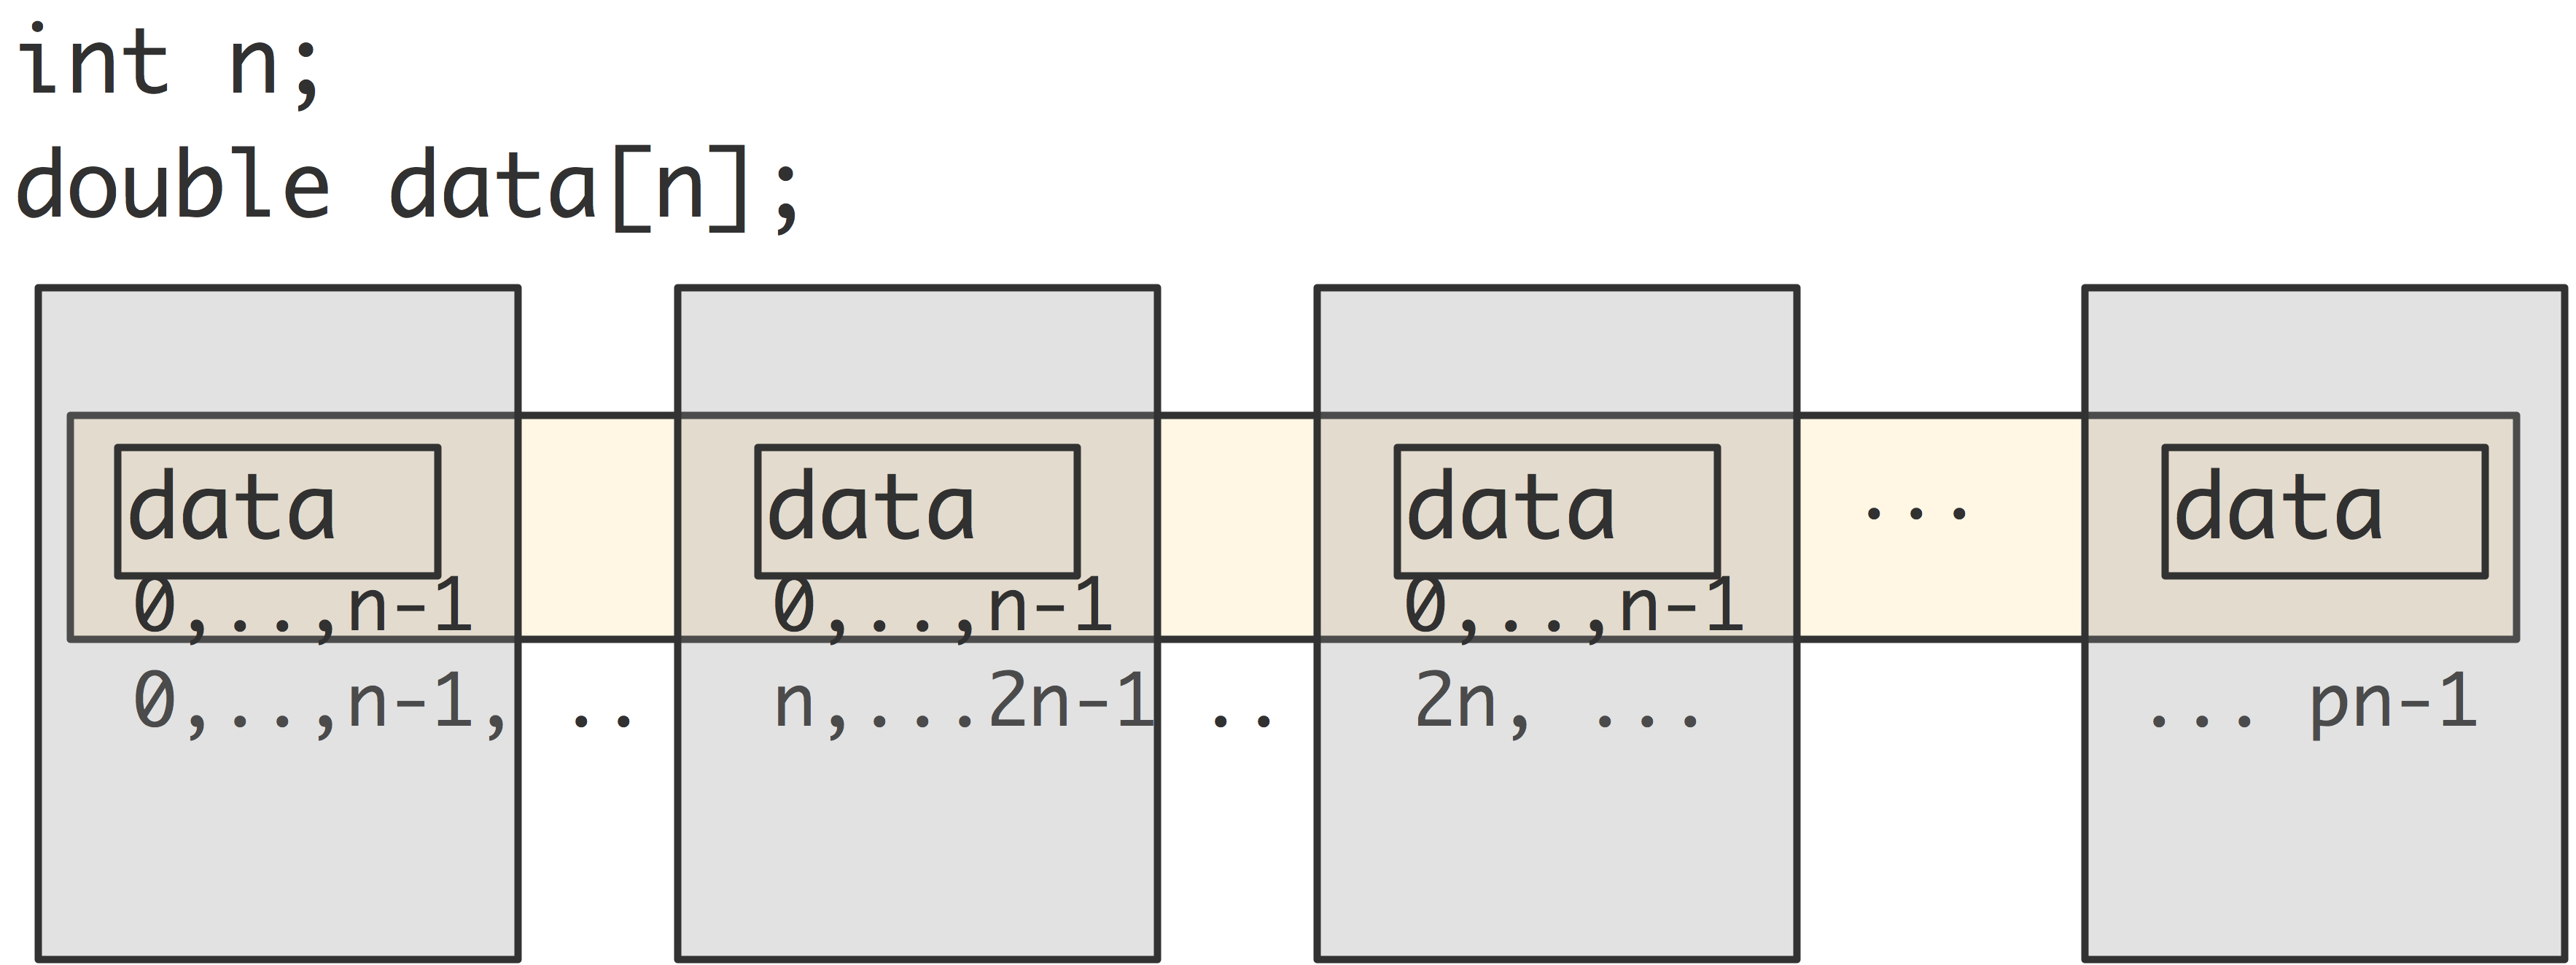
\includegraphics[scale=.1]{mpi-array}
  \caption{Local parts of a distributed array}
  \label{fig:mpi-array}
\end{figure}

We sometimes say that \n{data} is the local part
of a \indexterm{distributed array} with a total size of
$\n{n}\cdot\n{p}$ elements.
However, this array only exists
conceptually: each processor has an array with lowest index zero,
and you have to translate that yourself to an index in the global
array.
In other words, you have to write your code in such a way that
it acts like you're working with a large array that is distributed
over the processors, while
actually manipulating only the local arrays on the processors.

Your typical code then looks like
\begin{verbatim}
int myfirst = .....;
for (int ilocal=0; ilocal<nlocal; ilocal++) {
   int iglobal = myfirst+ilocal;
   array[ilocal] = f(iglobal);
}
\end{verbatim}

\begin{exercise}
  \label{ex:sumsquares}
  We want to compute $\sum_{n=1}^Nn^2$, and we do that as follows
  by filling in an array and summing the elements. (Yes, you can do it
  without an array, but for purposes of the exercise do it with.)

  Set a variable \n{N} for the total length of the array, and compute
  the local number of elements. Make sure you handle the case where
  $N$ does not divide perfectly by the number of processes.

  \begin{itemize}
  \item Now allocate the local parts: each processor should allocate
    only local elements, not the whole vector.\\
    (Allocate your array as real numbers. Why are integers not a good idea?)
  \item On each processor, initialize the local array
    so that the $i$-th location of the distributed array
    (for $i=0,\ldots,N-1$)
    contains~$(i+\nobreak 1)^2$.
  \item Now use a collective operation to compute the sum of the array values.
    The right value is $(2N^3+3N^2+N)/6$. Is that what you get?
  \end{itemize}
  (Note that computer arithmetic is not exact: the computed sum will
  only be accurate up to some relative accuracy.)
\end{exercise}

\begin{exercise}
  In exercise~\ref{ex:sumsquares} you worked with a distributed array,
  computing a local quantity and combining that into a global
  quantity.
  Why is it not a good idea to gather the whole distributed array on a
  single processor, and do all the computation locally?
\end{exercise}

If the array size is not perfectly divisible by the number of processors,
we have to come up with a division that is uneven, but not too much.
You could for instance, write
\begin{verbatim}
int Nglobal, // is something large
    Nlocal = Nglobal/ntids,
    excess = Nglobal%ntids;
if (mytid==ntids-1) 
  Nlocal += excess;
\end{verbatim}

\begin{exercise}
  Argue that this strategy is not optimal. Can you come up with a
  better distribution?
  Load balancing is further discussed in~\HPSCref{sec:load}.
\end{exercise}

One of the more common applications of the reduction operation
is the \indexterm{inner product} computation. Typically, you have two vectors $x,y$
that have the same distribution, that is,
where all processes store equal parts of $x$ and~$y$.
The computation is then
\begin{verbatim}
local_inprod = 0;
for (i=0; i<localsize; i++)
  local_inprod += x[i]*y[i];
MPI_Reduce( &local_inprod, &global_inprod, 1,MPI_DOUBLE ... ) 
\end{verbatim}
If all processors need the result, you could then do a broadcast,
but it is more efficient to use \indexmpishow{MPI_Allreduce}; 
see section~\ref{sec:allreduce}.

\begin{exercise}
  \label{ex:inproduct}
  Implement an inner product routine: let $x$ be a
  distributed vector of size~$N$ with elements $x[i]=i$,
  and compute~$x^tx$.
  As before, the right value is $(2N^3+3N^2+N)/6$.

  Use the inner product value to scale to vector so that it has
  norm~1.
  Check that your computation is correct.
\end{exercise}

%% \Level 0 {Blocking point-to-point operations}
\input chapters/mpi-blocksend

%% \Level 0 {Non-blocking point-to-point operations}
\input chapters/mpi-nonblock

\Level 0 {More about point-to-point communication}

\Level 1 {Message probing}

MPI receive calls specify a receive buffer, and its size has to be
enough for any data sent. In case you really have no idea how much data
is being sent, and you don't want to overallocate the receive buffer,
you can use a `probe' call.

The calls \indexmpishow{MPI_Probe}, \indexmpishow{MPI_Iprobe}, accept a message,
but do not copy the data. Instead, when probing tells you that there is a
message, you can use \indexmpishow{MPI_Get_count} to determine its size,
allocate a large enough receive buffer, and do a regular receive to
have the data copied.

\verbatimsnippet{probe}

\mpiRoutineRef{MPI_Probe}

There is a problem with the \indexmpishow{MPI_Probe} call: in a
multithreaded environment the following scenario can happen.
\begin{enumerate}
\item A thread determines by probing that a certain message has come
  in.
\item It issues a blocking receive call for that message\dots
\item But in between the probe and the receive call another thread
  has already received the message.
\item \dots~Leaving the first thread in a blocked state with not
  message to receive.
\end{enumerate}
This is solved by \indexmpishow{MPI_Mprobe}, which after a successful
probe removes the message from the \indexterm{matching queue}: the
list of messages that can be matched by a receive call. The thread
that matched the probe now issues an \indexmpishow{MPI_Mrecv} call on
that message through an object of type \indexmpidef{MPI_Message}.

\mpiRoutineRef{MPI_Mprobe}

\mpiRoutineRef{MPI_Mrecv}

\Level 1 {Wildcards in the receive call}
\label{sec:mpi-status}

With some receive calls you know everything about the message in advance:
its source, tag, and size. In other cases you want to leave some options
open, and inspect the message for them after it was received.
To do this, the receive call has a \emph{status}\index{status!of receive call}
parameter.
This status is a property of the actually received messsage, so \n{MPI_Irecv}
does not have a status parameter, but \n{MPI_Wait} does.

Here are some of the uses of the status:
\heading{Source} In some applications it makes sense that a message can come from 
one of a number of processes. In this case, it is possible to specify
\indexmpishow{MPI_ANY_SOURCE} as the source. To find out where the message actually
came from, you would use the \indexmpishow{MPI_SOURCE} field of the status object
that is delivered by \n{MPI_Recv} or the \n{MPI_Wait...} call after an \n{MPI_Irecv}.
\begin{verbatim}
MPI_Recv(recv_buffer+p,1,MPI_INT, MPI_ANY_SOURCE,0,comm,
         &status);
sender = status.MPI_SOURCE;
\end{verbatim}

There are various scenarios where receiving from `any source' makes sense.
One is that of the \indexterm{master-worker model}. The master task would first send
data to the worker tasks, then issues a blocking wait for the data of whichever process
finishes first.

If a processor is expecting more than one messsage from a single other processor,
message tags are used to distinguish between them. In that case,
a value of \indexmpishow{MPI_ANY_TAG} can be used, and the actual tag
of a message can be retrieved with
\begin{verbatim}
int tag = status.MPI_TAG;
\end{verbatim}

If the amount of data received is not known a~priori, the amount received
can be found as
\begin{verbatim}
MPI_Get_count(&recv_status,MPI_INT,&recv_count);
\end{verbatim}

\Level 1 {Synchronous and asynchronous communication}

\index{communication!synchronous|(textbf}
\index{communication!asynchronous|(textbf}

It is easiest to think of blocking as a form of synchronization with
the other process, but that is not quite true. Synchronization is a
concept in itself, and we talk about \emph{synchronous} communication
if there is actual coordination going on with the other process,
and \emph{asynchronous} communication if there is not. Blocking then
only refers to the program waiting until the user data is safe
to reuse; in the synchronous case a blocking call means that the data
is indeed transferred, in the asynchronous case it only means that the
data has been transferred to some system buffer.
%
\begin{figure}[ht]
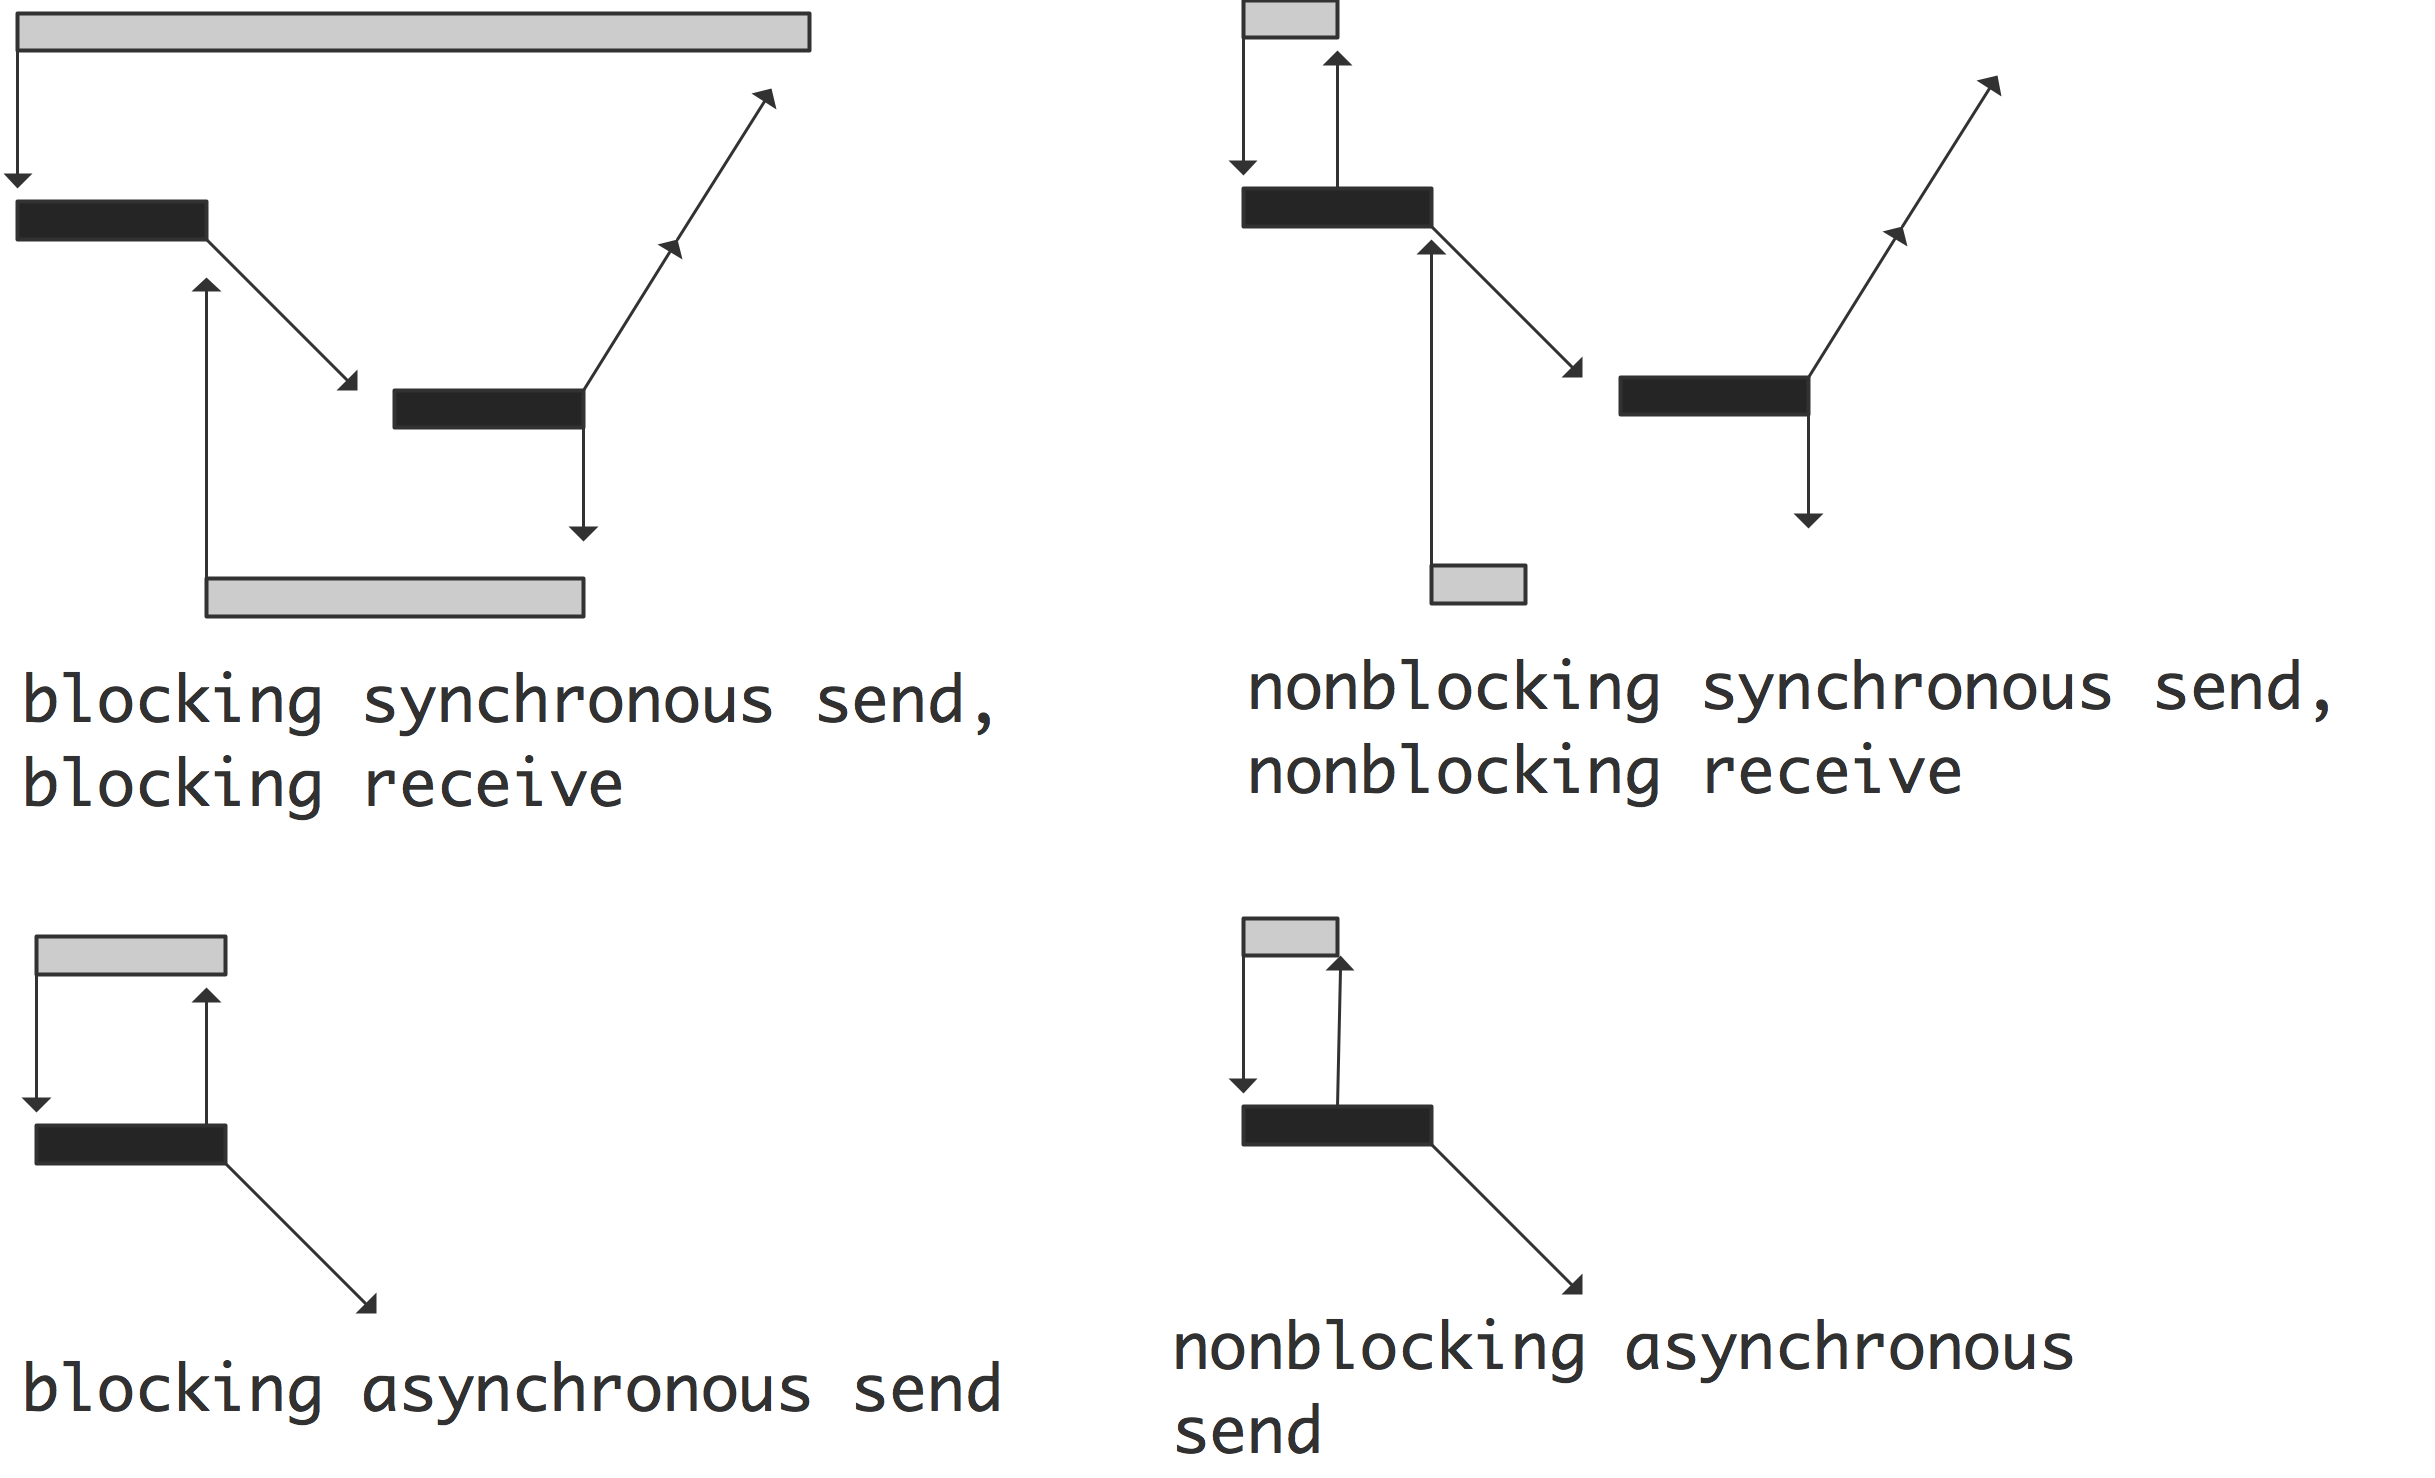
\includegraphics[scale=.15]{block-vs-sync}
\caption{Blocking and synchronicity}
\label{fig:block-sync}
\end{figure}
The four possible cases are illustrated in figure~\ref{fig:block-sync}.

MPI has a number of routines for synchronous communication,
such as \indexmpishow{MPI_Ssend}.

\index{communication!synchronous|)}
\index{communication!asynchronous|)}

\Level 1 {Buffered communication}
\label{sec:buffered}

By now you have probably got the notion that managing buffer
space in MPI is important: data has to be somewhere, either in
user-allocated arrays or in system buffers. Buffered sends are yet another
way of managing buffer space.
\begin{enumerate}
\item You allocate your own buffer space, and you attach it to your process;
\item You use the \indexmpishow{MPI_Bsend} call for sending;
\item You detach the buffer when you're done with the buffered sends.
\end{enumerate}

There can be only one buffer per process; its size should be enough
for all outstanding \indexmpishow{MPI_Bsend} calls that are simultaneously
outstanding, plus \indexmpishow{MPI_BSEND_OVERHEAD}.

\indexmpishow{MPI_Buffer_attach}
\begin{verbatim}
int MPI_Buffer_attach(
  void *buffer,int size);
\end{verbatim}
where the size is indicated in bytes.
The possible error codes are
\begin{itemize}
\item \n{MPI_SUCCESS} the routine completed successfully.
\item \indexmpishow{MPI_ERR_BUFFER} The buffer pointer is invalid;
  this typically means that you have supplied a null pointer.
\item \indexmpishow{MPI_ERR_INTERN} An internal error in MPI has been detected.
\end{itemize}

The buffer is detached with \indexmpishow{MPI_Buffer_detach}:
\begin{verbatim}
int MPI_Buffer_detach(
  void *buffer, int *size);
\end{verbatim}
This returns the address and size of the buffer; the call blocks
until all buffered messages have been delivered.

You can compute the needed size of the buffer with \indexmpishow{MPI_Pack_size};
see section~\ref{sec:pack}.

\indexmpishow{MPI_Bsend}
\begin{verbatim}
int MPI_Bsend(
  const void *buf, int count, MPI_Datatype datatype, 
  int dest, int tag, MPI_Comm comm)
\end{verbatim}
The asynchronous version is \indexmpishow{MPI_Ibsend}.

You can force delivery by
\begin{verbatim}
MPI_Buffer_detach( &b, &n );
MPI_Buffer_attach( b, n );
\end{verbatim}

\Level 1 {Persistent communication}
\label{sec:persistent}
\index{communication!persistent|(textbf}

An \n{Isend} or \n{Irecv} call has an \n{MPI_Request} parameter. This
is an object that gets created in the send/recv call, and deleted in
the wait call. You can imagine that this carries some overhead, and if
the same communication is repeated many times you may want to avoid
this overhead by reusing the request object.

To do this, MPI has \emph{persistent communication}:
\index{persistent communication|see{communication, persistent}}
\begin{itemize}
\item You describe the communication with
  \indexmpishow{MPI_Send_init}, which has the same calling sequence as
  \n{MPI_Isend}, or \indexmpishow{MPI_Recv_init}, which has the same
  calling sequence as \n{MPI_Irecv}.
\item The actual communication is performed by calling
  \indexmpishow{MPI_Start}, for a single request, or
  \indexmpishow{MPI_Startall} for an array or requests.
\item Completion of the communication is confirmed with
  \indexmpishow{MPI_Wait} or similar routines as you have seen in the
  explanation of non-blocking communication.
\item The wait call does not release the request object: that is done
  with \indexmpishow{MPI_Request_free}.
\end{itemize}

The calls \indexmpishow{MPI_Send_init} and \indexmpishow{MPI_Recv_init}
for creating a persistent communication have the same syntax as 
those for non-blocking sends and receives. The difference is that they do not start
an actual communication, they only create the request object.
%
\mpiRoutineRef{MPI_Send_init}
%
\mpiRoutineRef{MPI_Recv_init}
%

Given these request object, a communication (both send and receive) is then started
with \indexmpishow{MPI_Start} for a single request or \indexmpishow{MPI_Start_all} for 
multiple requests, given in an array.
\begin{verbatim}
int MPI_Start(MPI_Request *request)
\end{verbatim}
%
\mpiRoutineRef{MPI_Startall}
%
These are equivalent to starting an \n{Isend} or \n{Isend}; correspondingly, 
it is necessary to issue an \n{MPI_Wait...} call (section~\ref{ref:nonblocking})
to determine their completion.

After a request object has been used, possibly multiple times, it can be freed; see~\ref{ref:mpirequest}.

In the following example a ping-pong is implemented with persistent communication.
\verbatimsnippet{persist}

As with ordinary send commands, there are the variants
\indexmpishow{MPI_Bsend_init},
\indexmpishow{MPI_Ssend_init},
\indexmpishow{MPI_Rsend_init}.

\index{communication!persistent|)}

\Level 1 {About \texttt{MPI\_Request}}
\label{ref:mpirequest}

An \indexmpidef{MPI_Request} object is not actually an object,
unlike \n{MPI_Status}. Instead it is an (opaque) pointer.
This meeans that when you call, for instance, \n{MPI_Irecv},
MPI will allocate an actual request object, and return its
address in the \n{MPI_Request} variable.

Correspondingly, calls to \indexmpishow{MPI_Wait...} or \indexmpishow{MPI_Test}
free this object.
If your application is such that you do not use `wait' call, you can free the
request object explicitly
with \indexmpishow{MPI_Request_free}.
\begin{verbatim}
int MPI_Request_free(MPI_Request *request)
\end{verbatim}

You can inspect the status of a request without freeing the request object
with \indexmpishow{MPI_Request_get_status}:
\begin{verbatim}
int MPI_Request_get_status(
  MPI_Request request,
  int *flag,
  MPI_Status *status
);
\end{verbatim}

\index{communication!two-sided|)}

\endinput

%% \Level 0 {Shared-memory-like communication: one-sided
%% communication}
\input chapters/mpi-onesided

